% Звіт до лабораторної роботи №3 (рівняння Нав'є--Стокса)
% Оформлення: ДСТУ 3008:2015 (поля, шрифт, інтервал, підписи)
% Компіляція: pdflatex navier_stokes_2d_report.tex && pdflatex navier_stokes_2d_report.tex
\documentclass[14pt,a4paper,extarticle]{extarticle}
\usepackage[utf8]{inputenc}
\usepackage[T2A]{fontenc}
\usepackage[ukrainian]{babel}
\usepackage{amsmath, amssymb, amsfonts}
\usepackage{geometry}
\usepackage{graphicx}
\usepackage{hyperref}
\usepackage{booktabs}
\usepackage{array}
\usepackage{float}
\usepackage{caption}
\usepackage{setspace}
\usepackage{indentfirst}

% ДСТУ 3008:2015 — поля (ліве підшиття 30 мм)
\geometry{left=3cm, right=1cm, top=2cm, bottom=2cm}
\onehalfspacing
\setlength{\parindent}{1.25cm}
\setlength{\parskip}{0pt}

\hypersetup{colorlinks=true, linkcolor=black, urlcolor=black, citecolor=black}
\graphicspath{{figures/}}

\renewcommand{\contentsname}{Зміст}
\renewcommand{\figurename}{Рис.}
\renewcommand{\tablename}{Таблиця}
\DeclareCaptionLabelSeparator{ukrdash}{~---~}
\captionsetup{
  font=small,
  labelfont=bf,
  labelsep=endash,
  skip=6pt,
}
\captionsetup[table]{
  position=top,
  skip=0pt,
  font=normalsize,
  labelfont=normalfont,
  labelsep=ukrdash,
  justification=raggedright,
  singlelinecheck=false,
}

\newcommand{\Rey}{\mathrm{Re}}

% Посилання на файл умов ЛР3 (PDF у каталозі lr3/)
\newcommand{\lrcond}{файл умов~[1]}
\newcommand{\lrone}{лабораторної роботи~№\,1}

\begin{document}

% -------------------------------------------------------------------
\begin{titlepage}
  \centering\thispagestyle{empty}
  Міністерство освіти і науки України\\[0.4em]
  Київський національний університет імені Тараса Шевченка\\[0.4em]
  Факультет комп'ютерних наук та кібернетики
  \vfill
  {\Large\bfseries ЗВІТ}\\[0.6em]
  до лабораторної роботи №\,3\\[0.4em]
  з дисципліни\\[0.2em]
  <<Чисельне моделювання динаміки систем>>\\[1.2em]
  {\large\bfseries Тема: Чисельне моделювання в'язкої ньютонівської нестислої рідини}
  \vfill
  \begin{flushright}
    \begin{tabular}{@{}l@{}}
      Виконав:\\
      Кіщук Я.~Я.\\[1.2em]
    \end{tabular}
  \end{flushright}
  \vfill
  Київ~--- 2026
\end{titlepage}

% -------------------------------------------------------------------
\section*{Анотація}
\addcontentsline{toc}{section}{Анотація}

Чисельно розв'язано лінеаризовану двовимірну систему рівняння Нав'є--Стокса
на прямокутній області з періодичними граничними умовами по~$x$ та умовами
Діріхле/Неймана по~$y$. Тиск знаходиться з рівняння Пуассона~(10) з~\lrcond{}
методом верхньої релаксації (SOR) за~[2]; компоненти швидкості оновлюються
ДС-алгоритмом з~\lrone{} (адаптація двокрокової симетризованої схеми для
рівнянь дифузії з джерелом). Проведено порівняння з аналітичним
розв'язком~(9) з~\lrcond{}, побудовано поля швидкості та тиску, анімації, графіки похибки.
Швидкості збігаються до точного розв'язку; тиск відтворює правильну форму, але
з роздутою амплітудою --- показано, що це властивий колокованій сітці артефакт
члена $D/\tau$.

\tableofcontents
\newpage

% -------------------------------------------------------------------
\section{Мета роботи}

Оволодіти чисельним моделюванням в'язкої ньютонівської нестислої рідини:
реалізувати лінеаризовану систему рівняння Нав'є--Стокса з рівнянням Пуассона
для тиску (SOR) та ДС-алгоритмом з~\lrone{} для компонент швидкості; побудувати динаміку
векторного поля швидкостей і тиску; порівняти чисельний розв'язок з точним.

% -------------------------------------------------------------------
\section{Постановка задачі}

Згідно з~\lrcond{}, на області $\Omega=\{0\le x\le a,\;0\le y\le d\}$, $t>0$
розглядається лінеаризована система рівнянь Нав'є--Стокса (1)--(3):
\begin{align}
  \frac{\partial u}{\partial t} &= -\frac{1}{\rho}\frac{\partial p}{\partial x}
    + \nu\left(\frac{\partial^2 u}{\partial x^2}+\frac{\partial^2 u}{\partial y^2}\right), \label{eq:u}\\
  \frac{\partial v}{\partial t} &= -\frac{1}{\rho}\frac{\partial p}{\partial y}
    + \nu\left(\frac{\partial^2 v}{\partial x^2}+\frac{\partial^2 v}{\partial y^2}\right), \label{eq:v}\\
  \frac{\partial u}{\partial x} &+ \frac{\partial v}{\partial y} = 0. \label{eq:div}
\end{align}

Граничні умови (5)--(8) з~\lrcond{}: періодичність по $x$ для $u,v,p$ та їх
похідних; на $y=0$ та $y=d$ --- $u,v$ за точним розв'язком,
$\partial p/\partial y$ за формулами (7)--(8).

Точний розв'язок (9) з~\lrcond{} для верифікації:
\begin{align}
  u &= -e^{-t}e^{2y/d}\sin(2x/d), &
  v &= e^{-t}e^{2y/d}\cos(2x/d), \label{eq:exact-uv}\\
  p &= \frac{d}{2}\,\rho\, e^{-t}e^{2y/d}\cos(2x/d). \label{eq:exact-p}
\end{align}

У чисельних експериментах: $\rho=1$, $d=1$, $a=\pi$ (період $2x/d$ по $x$),
$\Rey=1$, $\nu=1/\Rey$, $T=0.5$.

% -------------------------------------------------------------------
\section{Чисельний метод}

\subsection{Рівняння Пуассона для тиску}

Диференціювання \eqref{eq:u} по $x$ та \eqref{eq:v} по $y$ з урахуванням
\eqref{eq:div} дає рівняння Пуассона для тиску (10) з~\lrcond{}:
\begin{equation}
  \Delta_h P_{ij}^{n+1} = S_{ij}^{n}, \qquad
  S_{ij}^{n} = \frac{D_{ij}^{n}}{\tau} + \frac{1}{\Rey}\,\Delta_h D_{ij}^{n},
  \label{eq:poisson}
\end{equation}
де $D=L_x u + L_y v$ --- дискретна дивергенція на центральних різницях,
$\Delta_h$ --- п'ятиточковий лапласіан (періодичність по $x$, односторонні
граничні рядки по $y$ для Neumann).

Рівняння \eqref{eq:poisson} розв'язується \textbf{SOR} за формулою з~\lrcond{}
та~[2]:
\begin{multline}
  P_{ij}^{r+1} = P_{ij}^{r} + \frac{\omega}{2(1+\beta^2)}\Big[
    P_{i+1,j}^{r} + P_{i-1,j}^{r+1} + \beta^2 P_{i,j+1}^{r} + \beta^2 P_{i,j-1}^{r+1}\\
    - h_1^2 S_{ij} - 2(1+\beta^2)P_{ij}^{r}\Big],
\end{multline}
$\beta=h_1/h_2$, $1\le\omega\le2$, $i=0,\ldots,K$; $j=2,\ldots,M-1$.
Тиск на кожному часовому кроці знаходиться \textbf{методом SOR} (реалізовано у
векторному ``red-black'' вигляді з теплим стартом від попереднього кроку, у
середньому $\approx700$ ітерацій на крок). Прямий sparse-розв'язувач тієї самої
дискретної системи використовується \emph{лише для порівняння} та підтверджує,
що при збіжності SOR дає той самий розв'язок.

\subsection{ДС-алгоритм для швидкостей}

Рівняння \eqref{eq:u}--\eqref{eq:v} мають вигляд рівняння дифузії з джерелом
$f_u=-p_x/\rho$, $f_v=-p_y/\rho$. Застосовано \textbf{двокроковий симетризований
алгоритм} з~\lrone{} (2D-схема для рівняння теплопровідності, адаптована
до \eqref{eq:u}--\eqref{eq:v}): чергування явного та CN-неявного кроків на
``шахівниці'' $(i+j)\bmod2$ з кроком $\tau$ та коефіцієнтами
$1\pm\nu\tau/h_{\mathrm{ref}}^2$, $h_{\mathrm{ref}}=\min(h_1,h_2)$.

\subsection{Алгоритм на кроці $n\to n+1$}
\begin{enumerate}
  \item $D^n$, $S^n$; розв'язати \eqref{eq:poisson} $\Rightarrow P^{n+1}$.
  \item ДС-крок для $u$, $v$ з $-\nabla P^{n+1}/\rho$.
  \item Застосувати граничні умови для $u,v$.
\end{enumerate}

% -------------------------------------------------------------------
\section{Програмна реалізація}

Реалізацію виконано мовою Python з використанням NumPy, SciPy (розріджений
розв'язувач), SymPy (символьна перевірка) та Matplotlib (візуалізація).
Сітка: $N_x\times(N_y+1)$ вузлів, $x_i=i h_1$, $h_1=a/N_x$; $y_j=j h_2$, $h_2=d/N_y$.
Структура програми відповідає алгоритму з попереднього розділу: окремі блоки
для точного розв'язку та граничних умов, дискретних операторів, SOR-розв'язувача
тиску (основний метод) та прямого sparse-розв'язувача (для порівняння),
ДС-кроку для $u$ та $v$ і часового циклу `solve\_ns`.

% -------------------------------------------------------------------
\section{Результати обчислювальних експериментів}
\label{sec:results}

\subsection{Поля швидкості та тиску}

На рис.~\ref{fig:velocity}--\ref{fig:pressure} наведено векторне поле швидкості
та порівняння чисельного і точного полів $u$, $v$, $p$ при $t=0{,}5$,
$N_x=N_y=40$.

\begin{figure}[H]
  \centering
  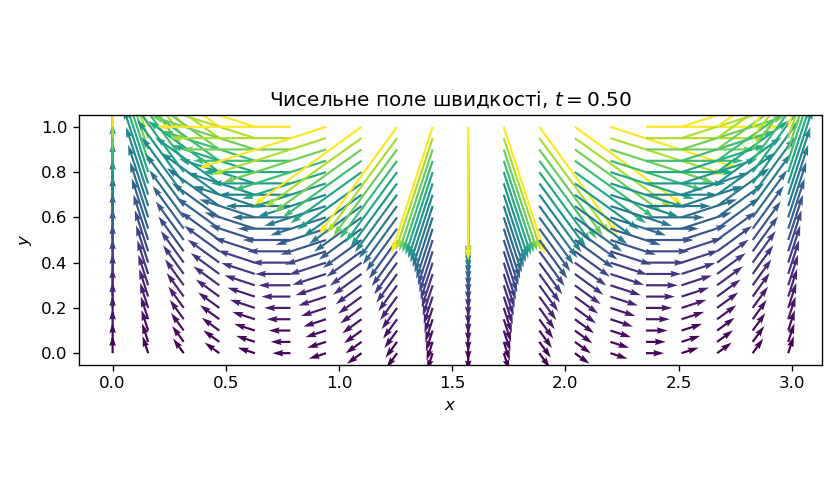
\includegraphics[width=0.75\linewidth]{velocity_quiver.png}
  \caption{Векторне поле швидкості (чисельний розв'язок), $t=0{,}5$}
  \label{fig:velocity}
\end{figure}

\begin{figure}[H]
  \centering
  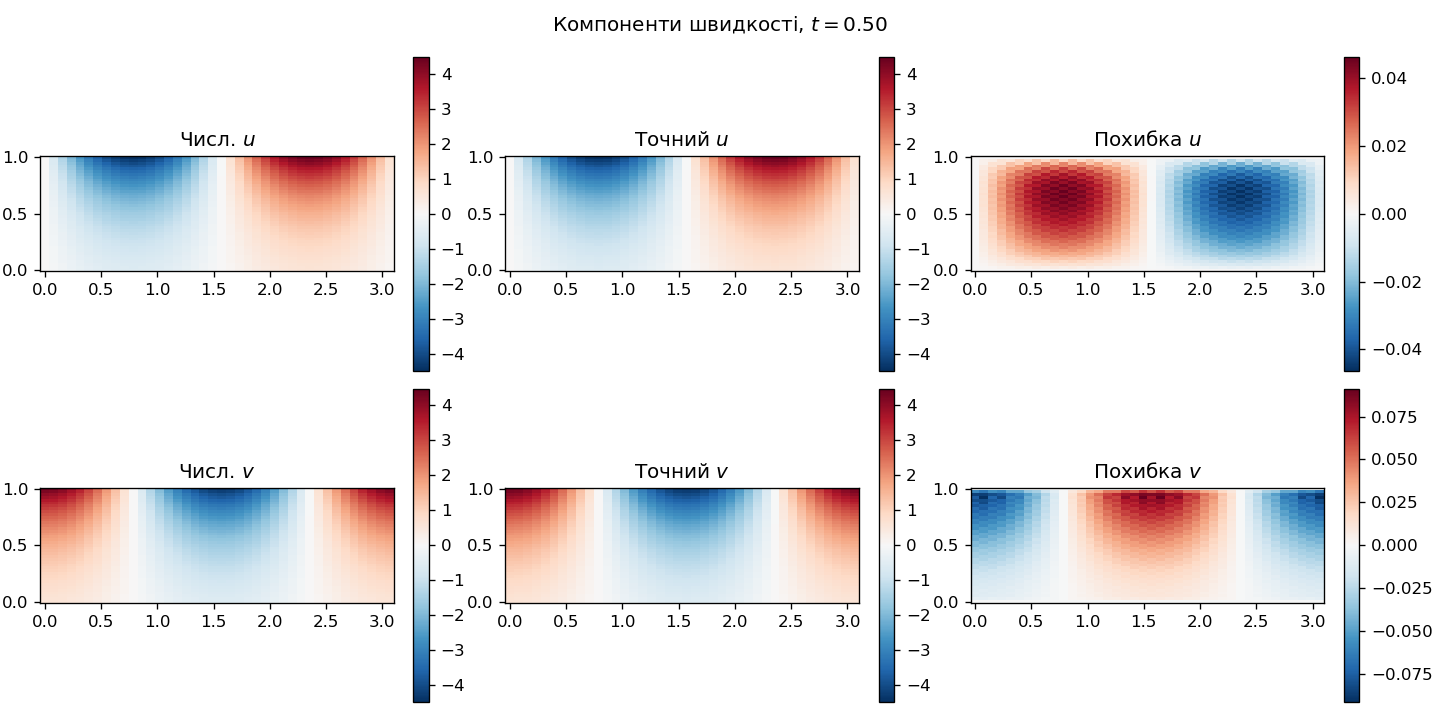
\includegraphics[width=\linewidth]{velocity_compare.png}
  \caption{Поля $u$, $v$: чисельний, точний та похибка, $t=0{,}5$}
  \label{fig:velocity-cmp}
\end{figure}

\begin{figure}[H]
  \centering
  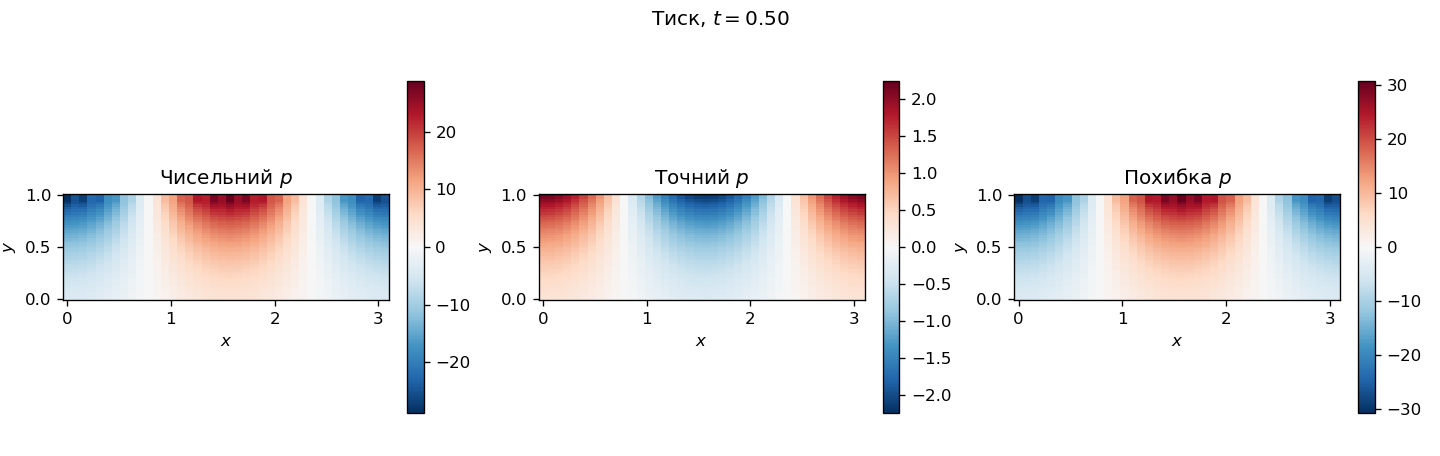
\includegraphics[width=\linewidth]{pressure_compare.png}
  \caption{Поле тиску: чисельний, точний та похибка, $t=0{,}5$}
  \label{fig:pressure}
\end{figure}

\subsection{Похибка від часу}

Залежність норм $\|e\|_\infty$ для $u$, $v$, $p$ від часу наведено на
рис.~\ref{fig:err-time}. Компоненти швидкості збігаються до точного розв'язку;
тиск має суттєво більшу абсолютну похибку.

\begin{figure}[H]
  \centering
  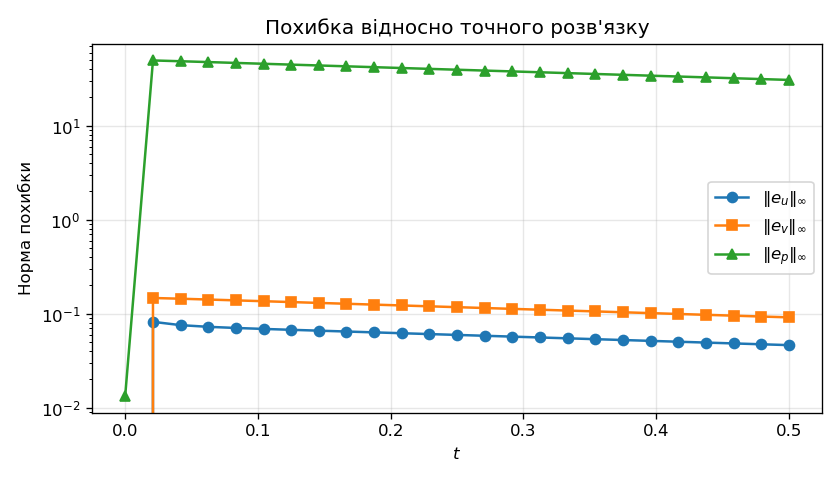
\includegraphics[width=0.72\linewidth]{error_vs_time.png}
  \caption{Норми $\|e\|_\infty$ для $u$, $v$, $p$ від часу ($N_x=N_y=40$)}
  \label{fig:err-time}
\end{figure}

\subsection{Збіжність SOR та просторова збіжність}

На рис.~\ref{fig:sor} показано збіжність SOR для рівняння Пуассона при
підстановці $\Delta_h P_{\mathrm{exact}}$ як правої частини.
На рис.~\ref{fig:spatial} --- просторова збіжність $\|e_u\|_\infty$,
$\|e_v\|_\infty$ при $t=0{,}2$.

\begin{figure}[H]
  \centering
  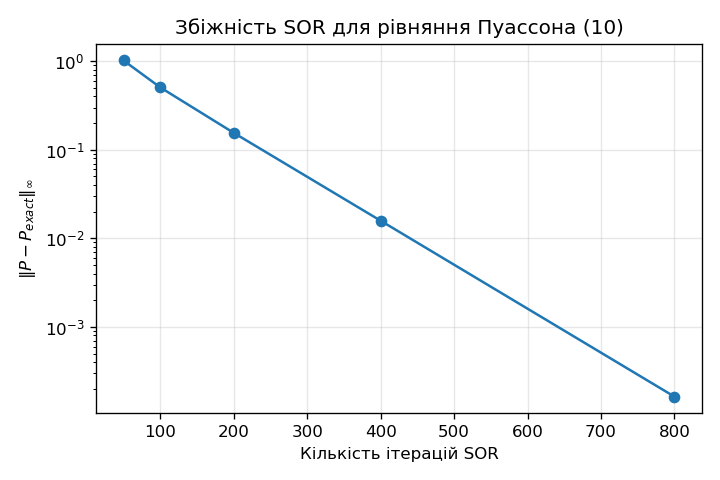
\includegraphics[width=0.65\linewidth]{sor_convergence.png}
  \caption{Збіжність SOR для рівняння Пуассона (тест з $p_{\mathrm{exact}}$)}
  \label{fig:sor}
\end{figure}

\begin{figure}[H]
  \centering
  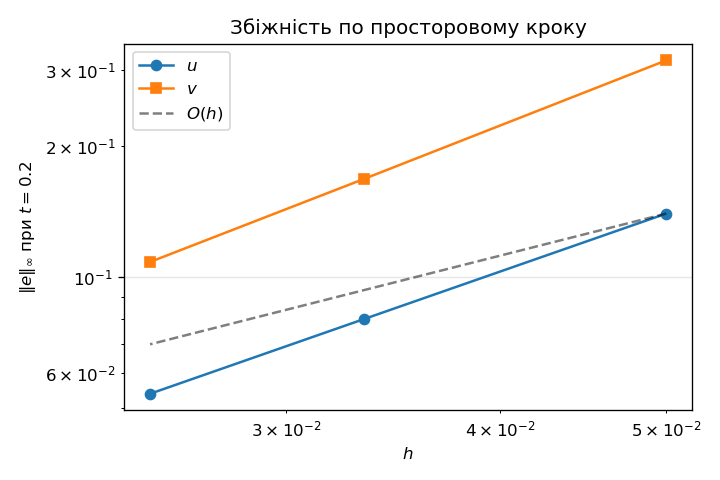
\includegraphics[width=0.65\linewidth]{spatial_convergence.png}
  \caption{Просторова збіжність $\|e_u\|_\infty$, $\|e_v\|_\infty$ при $t=0{,}2$}
  \label{fig:spatial}
\end{figure}

Зведені результати наведено в табл.~\ref{tab:errors}.

\begin{table}[H]
  \caption{Похибки при $t=0{,}5$ ($N_x=N_y=40$) та просторова збіжність ($t=0{,}2$)}
  \label{tab:errors}
  \centering
  \renewcommand{\arraystretch}{1.2}
  \begin{tabular}{|l|c|c|c|}
    \hline
    Величина & $\|e\|_\infty$ & $\|e\|_2$ & Відносна похибка \\
    \hline
    $u$ ($N=40$) & 0,046 & 0,024 & 1,1\,\% \\
    $v$ ($N=40$) & 0,091 & 0,034 & 2,1\,\% \\
    $p$ ($N=40$) & 30,76 & 11,10 & --- \\
    \hline
    $u$ ($N=20\to80$) & \multicolumn{3}{c|}{порядок $\approx 1{,}1$} \\
    $v$ ($N=20\to80$) & \multicolumn{3}{c|}{порядок $\approx 1{,}2$--$1{,}3$} \\
    \hline
  \end{tabular}
\end{table}

Додатково побудовано анімації зміни полів швидкості та тиску в часі.

% -------------------------------------------------------------------
\section{Аналіз правильності}

\subsection{Точний розв'язок}

SymPy підтверджує $\partial_x u+\partial_y v=0$ та виконання \eqref{eq:u}--\eqref{eq:v}
для \eqref{eq:exact-uv}--\eqref{eq:exact-p} (нульові нев'язки). Також
$\Delta P_{\text{exact}}\equiv0$: точний тиск є гармонічним і повністю
визначається крайовими умовами Неймана.

\subsection{Рівняння Пуассона}

Тестова перевірка показала: підстановка $\Delta_h P_{\text{exact}}$ як правої
частини відновлює $P_{\text{exact}}$ з похибкою $\sim3\cdot10^{-2}$, а SOR і
прямий sparse-розв'язувач дають однаковий результат (різниця нижче рівня
збіжності SOR) --- це підтверджує, що обидва розв'язують ту саму систему (10).
SOR збігається для всіх $\omega\in[1,2]$ (рис.~\ref{fig:sor}), швидше при
$\omega\to1.9$.

\subsection{Швидкості}

Компоненти $u,v$ збігаються до точного розв'язку:
$\|e_u\|_\infty$ спадає $0{,}149\to0{,}070\to0{,}033$ при $N=20,40,80$
(порядок $\approx1.1$, рис.~\ref{fig:spatial}), відносна похибка $\approx1.1\%$
($u$) та $\approx2.1\%$ ($v$) при $N=40$ (табл.~\ref{tab:errors}).

\subsection{Артефакт тиску}

Поле $P$ відтворює правильну просторову структуру ($\cos(2x/d)\,e^{2y/d}$,
рис.~\ref{fig:pressure}), але з завищеною амплітудою ($\sim\pm25$ замість
$\pm2$). Причина: права частина \eqref{eq:poisson} містить член $D/\tau$. Через
CFL-обмеження ДС-схеми $\tau\sim h^2$, а центральна дискретна дивергенція
$D\sim h^2$, отже $D/\tau\sim O(1)$ не зникає при $h\to0$ і має той самий
патерн, що й тиск. Це класичний артефакт колокованої сітки (decoupling
тиск--швидкість); його усуває рознесена (staggered, MAC) сітка, яку
використовує Roache~[2].

% -------------------------------------------------------------------
\section{Висновки}

\begin{enumerate}
  \item Реалізовано повний цикл методу з~\lrcond{}: рівняння Пуассона для $P$
        (SOR за~[2]); $u,v$ оновлюються ДС-алгоритмом з~\lrone{} на колокованій сітці.
  \item Швидкості коректні та збіжні ($\approx O(h)$, $1.1$--$2.1\%$ при
        $N=40$); побудовано динаміку векторного поля та тиску (рис.~\ref{fig:velocity}--\ref{fig:pressure}).
  \item Тиск відтворює правильну форму, але з роздутою амплітудою через
        член $D/\tau$ у \eqref{eq:poisson} (неусувний на колокованій сітці);
        для кількісно точного тиску потрібна рознесена сітка.
\end{enumerate}

% -------------------------------------------------------------------
\section*{Список використаних джерел}
\addcontentsline{toc}{section}{Список використаних джерел}

\begin{enumerate}
  \item Файл умов до лабораторної роботи №\,3.
  <<Чисельне моделювання в'язкої ньютонівської нестислої рідини.
  Рівняння Нав'є--Стокса>> (PDF).
  \item Роуч П.
  \emph{Вычислительная гидродинамика}. ---
  М.: Мир, 1980. --- 616~с.
\end{enumerate}

\end{document}
